\documentclass{article}
\usepackage[utf8]{inputenc}
\usepackage[T1]{fontenc}
\usepackage{booktabs}
\usepackage{graphicx}
\usepackage{hyperref}
\usepackage{xcolor}
\definecolor{validated}{HTML}{047857}
\definecolor{refuted}{HTML}{B91C1C}
\definecolor{inconclusive}{HTML}{9A3412}
\title{Audit Record}
\date{2026-05-15T13:54:11.905265+00:00}
\begin{document}
\maketitle
\section*{Audit Record}
\textbf{Audit ID:} \texttt{422dabe1a803e2ec9113e56bbcd47dda\dots}\\
\textbf{Captured:} 2026-05-15T13:54:11.905265+00:00\\
\textbf{Target:} \texttt{/Volumes/Behemoth/Ophamin FrameWork /ophamin/src/ophamin}
\subsection*{1. Pillars}
\begin{tabular}{llllrr}\toprule
\textbf{Pillar} & \textbf{Tool} & \textbf{Version} & \textbf{Status} & \textbf{Findings} & \textbf{Wall-time (s)} \\\midrule
\texttt{ruff} & \texttt{ruff} & ruff 0.15.7 & ok & 13 & 0.02 \\
\texttt{bandit} & \texttt{bandit} & bandit 1.9.3 & ok & 40 & 0.42 \\
\texttt{mypy} & \texttt{mypy} & mypy 1.19.1 (compiled: yes) & ok & 57 & 2.87 \\
\texttt{vulture} & \texttt{vulture} &  & unavailable & 0 & 0.00 \\
\texttt{radon} & \texttt{radon} &  & unavailable & 0 & 0.00 \\
\texttt{pip\_audit} & \texttt{pip-audit} &  & unavailable & 0 & 0.00 \\
\bottomrule\end{tabular}
\subsection*{2. Summary}
Total findings: \textbf{110}\\
\begin{figure}[h!]\centering
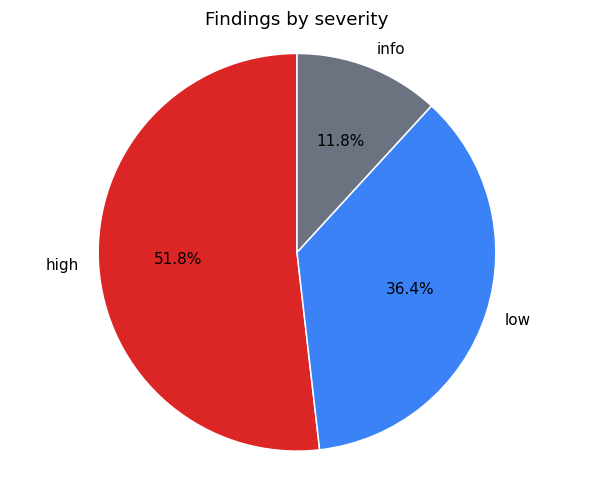
\includegraphics[width=0.55\linewidth]{assets/severity}
\caption{Findings by severity.}\end{figure}
\begin{figure}[h!]\centering
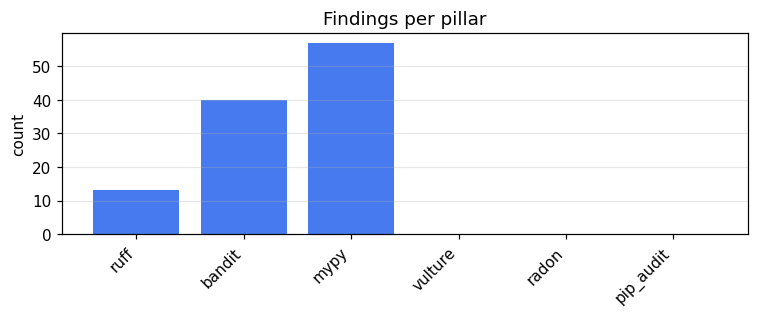
\includegraphics[width=0.7\linewidth]{assets/per_pillar}
\caption{Findings per pillar.}\end{figure}
\begin{figure}[h!]\centering
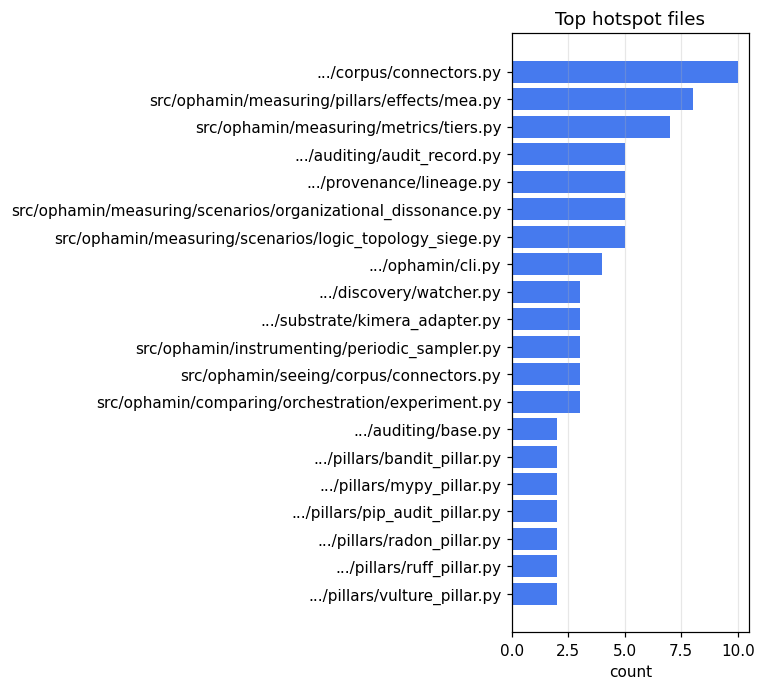
\includegraphics[width=0.85\linewidth]{assets/hotspots}
\caption{Top hotspot files by finding count.}\end{figure}
\subsection*{3. Signature}
\texttt{3a9f086d7c397802cc146e61e19f7abbc1dada18dea77e12e9d6b56fb3945e28}\\

\end{document}
